\documentclass[10pt, twocolumn, twoside, letterpaper]{IEEEtran}

\usepackage[activate={true, nocompatibility}, final, tracking=true, kerning=true, spacing=true, factor=1100, stretch=10, shrink=10]{microtype}
\linespread{0.9}

\makeatletter
\def\ps@IEEEtitlepagestyle{
  \def\@oddfoot{\mycopyrightnotice}
  \def\@evenfoot{}
}

\def\mycopyrightnotice{
  {\footnotesize
  \begin{minipage}{\textwidth}
  \centering
  978-1-7281-4164-0/19/\$31.00 \copyright2019 IEEE
  \end{minipage}
  }
}

\ifCLASSINFOpdf
   \usepackage[pdftex]{graphicx}
\else
   \usepackage[dvips]{graphicx}
\fi

\ifCLASSOPTIONcompsoc
  \usepackage[caption=false, font=normalsize, labelfont=sf, textfont=sf]{subfig}
\else
  \usepackage[caption=false, font=footnotesize]{subfig}
\fi

\usepackage{amsmath}
\usepackage{bm}
\usepackage{amssymb}
\usepackage{algorithm}
\usepackage{algorithmic}
\usepackage{stfloats}
\usepackage{url}
\usepackage{siunitx}
\usepackage{fancyref}

\usepackage{geometry}
\geometry{letterpaper, top=0.7in, bottom=0.7in, left=0.65in, right=0.65in}

\usepackage[acronym, nomain]{glossaries}

% Define "long-s" key: 
\glsaddkey* {longs}% key 
{\glsentrylong{\glslabel}s}% default value 
{\glsentrylongs}% command analogous to \glsentrytext 
{\Glsentrylongs}% command analogous to \Glsentrytext 
{\glslongs}% command analogous to \glstext 
{\Glslongs}% command analogous to \Glstext 
{\GLSlongs}% command analogous to \GLStext

%% Define "short-s" key: 
\glsaddkey* {shorts}% key 
{\glsentryshort{\glslabel}s}% default value 
{\glsentryshorts}% command analogous to \glsentrytext 
{\Glsentryshorts}% command analogous to \Glsentrytext 
{\glsshorts}% command analogous to \glstext 
{\Glsshorts}% command analogous to \Glstext 
{\GLSshorts}% command analogous to \GLStext

\DeclareRobustCommand{\glss}[1]
{%
  \ifglsused{#1}{\glsshorts{#1}}{\glslongs{#1} (\glsshorts{#1})\glsunset{#1}}%
}

\DeclareRobustCommand{\Glss}[1]
{%
  \ifglsused{#1}{\Glsshorts{#1}}{\Glslongs{#1} (\glsshorts{#1})\glsunset{#1}}%
}

% Define "long-ing" key: 
\glsaddkey* {longing}% key 
{\glsentrylong{\glslabel}ing}% default value 
{\glsentrylonging}% command analogous to \glsentrytext 
{\Glsentrylonging}% command analogous to \Glsentrytext 
{\glslonging}% command analogous to \glstext 
{\Glslonging}% command analogous to \Glstext 
{\GLSlonging}% command analogous to \GLStext

%% Define "short-ing" key: 
\glsaddkey* {shorting}% key 
{\glsentryshort{\glslabel}ing}% default value 
{\glsentryshorting}% command analogous to \glsentrytext 
{\Glsentryshorting}% command analogous to \Glsentrytext 
{\glsshorting}% command analogous to \glstext 
{\Glsshorting}% command analogous to \Glstext 
{\GLSshorting}% command analogous to \GLStext

\DeclareRobustCommand{\glsing}[1]
{%
  \ifglsused{#1}{\glsshorting{#1}}{\glslonging{#1} (\glsshorting{#1})\glsunset{#1}}%
}

\DeclareRobustCommand{\Glsing}[1]
{%
  \ifglsused{#1}{\Glsshorting{#1}}{\Glslonging{#1} (\glsshorting{#1})\glsunset{#1}}%
}

% Define "long-ed" key: 
\glsaddkey* {longed}% key 
{\glsentrylong{\glslabel}ed}% default value 
{\glsentrylonged}% command analogous to \glsentrytext 
{\Glsentrylonged}% command analogous to \Glsentrytext 
{\glslonged}% command analogous to \glstext 
{\Glslonged}% command analogous to \Glstext 
{\GLSlonged}% command analogous to \GLStext

%% Define "short-ed" key: 
\glsaddkey* {shorted}% key 
{\glsentryshort{\glslabel}ed}% default value 
{\glsentryshorted}% command analogous to \glsentrytext 
{\Glsentryshorted}% command analogous to \Glsentrytext 
{\glsshorted}% command analogous to \glstext 
{\Glsshorted}% command analogous to \Glstext 
{\GLSshorted}% command analogous to \GLStext

\DeclareRobustCommand{\glsed}[1]
{%
  \ifglsused{#1}{\glsshorted{#1}}{\glslonged{#1} (\glsshorted{#1})\glsunset{#1}}%
}

\DeclareRobustCommand{\Glsed}[1]
{%
  \ifglsused{#1}{\Glsshorted{#1}}{\Glslonged{#1} (\glsshorted{#1})\glsunset{#1}}%
}

\newacronym[longs={Motion Compensated Images}, shorts={MCIRs}]{MCI}{MCI}{Motion Compensated Image}
\newacronym[longs={Motion Compensated Image Reconstructions}, shorts={MCIRs}, longing={Motion Compensated Image Reconstructing}, shorting={MCIRing}, longed={Motion Compensated Image Reconstructed}, shorted={MCIRed}]{MCIR}{MCIR}{Motion Compensated Image Reconstruction}

\newacronym{1D}{1D}{$1$-Dimensional}
\newacronym{2D}{2D}{$2$-Dimensional}
\newacronym{3D}{3D}{$3$-Dimensional}
\newacronym[longs={$3$-Dimensional Point Clouds}, shorts={3DPCs}]{3DPC}{3DPC}{$3$-Dimensional Point Cloud}
\newacronym{4D}{4D}{$4$-Dimensional}
\newacronym{4DCT}{4DCT}{$4$-Dimensional Computed Tomography}
\newacronym[longs={Attenuation Corrections}, shorts={ACs}, longing={Attenuation Correcting}, shorting={ACing}, longed={Attenuation Corrected}, shorted={ACed}]{AC}{AC}{Attenuation Correct}
\newacronym[longs={Affine Deformations}, shorts={ADs}, longing={Affine Deforming}, shorting={ADing}, longed={Affine Deformed}, shorted={ADed}]{AD}{AD}{Affine Deformation}
\newacronym{AP}{AP}{Anterior Posterior}
\newacronym{ATP}{ATP}{Adenosine Triphosphate}
\newacronym[longs={B-Splines}, shorts={BSs}, longing={B-Splining}, shorting={BSing}, longed={B-Splined}, shorted={BSed}]{BS}{BS}{B-Spline}
\newacronym[longs={Cross Correlations}, shorts={CCs}, longing={Cross Correlating}, shorting={CCing}, longed={Cross Correlated}, shorted={CCed}]{CC}{CC}{Cross Correlation}
\newacronym{CCT}{CCT}{Cine Computed Tomography}
\newacronym{CG}{CG}{Conjugate Gradient}
\newacronym{COM}{COM}{Centre of Mass}
\newacronym[longs={Control Points}, shorts={CPs}]{CP}{CP}{Control Point}
\newacronym[longs={Control Point Grids}, shorts={CPGs}]{CPG}{CPG}{Control Point Grid}
\newacronym{CT}{CT}{Computed Tomography}
\newacronym{DD}{DD}{Data Driven}
\newacronym{DDG}{DDG}{Data Driven Gating}
\newacronym[longs={Deformation Vector Fields}, shorts={DVFs}]{DVF}{DVF}{Deformation Vector Field}
\newacronym{EM}{EM}{Expectation Maximisation}
\newacronym{FDG}{FDG}{Fludeoxyglucose}
\newacronym{F-FDG}{F-FDG}{Fluorine-$18$ Fludeoxyglucose}
\newacronym[longs={Fields of View}, shorts={FOVs}]{FOV}{FOV}{Field Of View}
\newacronym{FWHM}{FWHM}{Full Width at Half Maximum}
\newacronym{GD}{GD}{Gradient Descent}
\newacronym{GE}{GE}{General Electric}
\newacronym[longs={Ground Truths}, shorts={GTs}]{GT}{GT}{Ground Truth}
\newacronym[longs={Hounsfield Units}, shorts={HUs}]{HU}{HU}{Hounsfield Unit}
\newacronym[longs={Image Registrations}, shorts={IRs}, longing={Image Registering}, shorting={IRing}, longed={Image Registered}, shorted={IRed}]{IR}{IR}{Image Registration}
\newacronym[longs={Kilo Becquerel per Millilitres}, shorts={KBq/mLs}]{KBq/mL}{KBq/mL}{Kilo Becquerel per Millilitre}
\newacronym[longs={Kilo Electron Volts}, shorts={KeVs}]{KeV}{KeV}{Kilo Electron Volt}
\newacronym[longs={Kilo Volt}, shorts={KVs}]{KV}{KV}{Kilo Volt}
\newacronym[longs={Light Emitting Diodes}, shorts={LEDs}]{LED}{LED}{Light Emitting Diode}
\newacronym[longs={Lines of Responce}, shorts={LORs}]{LOR}{LOR}{Line of Response}
\newacronym[longs={Mean Absolute Errors}, shorts={MAEs}]{MAE}{MAE}{Mean Absolute Error}
\newacronym{MAPE}{MAPE}{Mean Absolute Percentage Error}
\newacronym{MBF}{MBF}{Myocardial Blood Flow}
\newacronym[longs={Motion Corrections}, shorts={MCs}, longing={Motion Correcting}, shorting={MCing} longed={Motion Corrected}, shorted={MCed}]{MC}{MC}{Motion Correction}
\newacronym{MI}{MI}{Mutual Information}
\newacronym{ML}{ML}{Maximum Likelihood}
\newacronym{MLAA}{MLAA}{Maximum Likelihood Reconstruction of Activity and Attenuation}
\newacronym{MLE}{MLE}{Maximum Likelihood Estimation}
\newacronym{MLEM}{MLEM}{Maximum Likelihood Expectation Maximisation}
\newacronym[longs={Motion Models}, shorts={MMs}, longing={Motion Modelling}, shorting={MMing}, longed={Motion Modelled}, shorted={MMed}]{MM}{MM}{Motion Model}
\newacronym[longs={Myocardial Perfusion Images}, shorts={MPIs}, longing={Myocardial Perfusion Imaging}, shorting={MPIing}, longed={Myocardial Perfusion Imaged}, shorted={MPIed}]{MPI}{MPI}{Myocardial Perfusion Image}
\newacronym{MR}{MR}{Magnetic Resonance}
\newacronym[longs={Mean Squared Errors}, shorts={MSEs}]{MSE}{MSE}{Mean Squared Error}
\newacronym[longs={Attenuation Maps}, shorts={Mu-Maps}]{Mu-Map}{Mu-Map}{Attenuation Map}
\newacronym[longs={Non-Attenuation Corrections}, shorts={NACs}, longing={Non-Attenuation Correcting}, shorting={NACing}, longed={Non-Attenuation Corrected}, shorted={NACed}]{NAC}{NAC}{Non-Attenuation Correct}
\newacronym{NMI}{NMI}{Normalised Mutual Information}
\newacronym{ND}{ND}{$n$-Dimensional}
\newacronym[longs={Non-Rigid Deformations}, shorts={NRDs}, longing={Non-Rigid Deforming}, shorting={NRDing}, longed={Non-Rigid Deformed}, shorted={NRed}]{NRD}{NRD}{Non-Rigid Deformation}
\newacronym{NTOF}{NTOF}{Non-Time of Flight}
\newacronym{OSEM}{OSEM}{Ordered Subset Expectation Maximisation}
\newacronym[longs={Principal Components}, shorts={PCs}]{PC}{PC}{Principal Component}
\newacronym{PCA}{PCA}{Principal Component Analysis}
\newacronym{PET}{PET}{Positron Emission Tomography}
\newacronym{PSMA}{PSMA}{Prostate Specific Membrane Antigen}
\newacronym[longs={Respiratory Correspondence Models}, shorts={RCMs}, longing={Respiratory Correspondence Modelling}, shorting={RCMing}, longed={Respiratory Correspondence Modelled}, shorted={RCMed}]{RCM}{RCM}{Respiratory Correspondence Model}
\newacronym[longs={Rigid Deformations}, shorts={RDs}, longing={Rigid Deforming}, shorting={RDing}, longed={Rigid Deformed}, shorted={RDed}]{RD}{RD}{Rigid Deformation}
\newacronym{RDP}{RDP}{Relative Difference Prior}
\newacronym[longs={Respiratory Motions}, shorts={RMs}]{RM}{RM}{Respiratory Motion}
\newacronym[longs={Regions of Interest}, shorts={ROIs}]{ROI}{ROI}{Region of Interest}
\newacronym{RPM}{RPM}{Real Time Position Management}
\newacronym{SGD}{SGD}{Stochastic Gradient Descent}
\newacronym{SI}{SI}{Superior Inferior}
\newacronym{SIRF}{SIRF}{Synergistic Image Reconstruction Framework}
\newacronym[longs={Signal to Noise Ratios}, shorts={SNRs}]{SNR}{SNR}{Signal to Noise Ratio}
\newacronym[longs={Surrogate Signals}, shorts={SSs}]{SS}{SS}{Surrogate Signal}
\newacronym{SSD}{SSD}{Sum of Squared Differences}
\newacronym{STIR}{STIR}{Software for Tomographic Image Reconstruction}
\newacronym[longs={Standard Uptake Values}, shorts={SUVs}]{SUV}{SUV}{Standard Uptake Value}
\newacronym{SVD}{SVD}{Singular Value Decomposition}
\newacronym{TOF}{TOF}{Time of Flight}
\newacronym[longs={Thin Plate Splines}, shorts={TPSs}]{TPS}{TPS}{Thin Plate Spline}
\newacronym{XCAT}{XCAT}{$4$-Dimensional Extended Cardiac Torso}

\usepackage[style=ieee, doi=false, isbn=false, url=false, maxbibnames=1, minbibnames=1, maxcitenames=1, mincitenames=1, backend=biber, defernumbers=false]{biblatex}
\addbibresource{./bibtex/bib/Biblio.bib}

\IEEEpubid{\begin{minipage}{\textwidth}\ \\[9pt] \centering
\medskip
\\
978-1-7281-2260-1/19/\$31.00~\copyright~2019~IEEE
\end{minipage}}

\begin{document}
\title{PET/CT Respiratory Motion Correction using NAC Derived Deformation Fields to Warp and Attenuation Correct with a single Attenuation Map}

\pagestyle{plain}
\pagenumbering{gobble}

\author{Alexander~C.~Whitehead,~\IEEEmembership{Student~Member,~IEEE,}
        Scott~W.~Wollenweber,~\IEEEmembership{Senior~Member~IEEE,}
        Charles~W.~Stearns,~\IEEEmembership{Fellow,~IEEE,}
        Brian~F.~Hutton,~\IEEEmembership{Senior~Member,~IEEE,}
        Jamie~R.~McClelland
        and~Kris~Thielemans,~\IEEEmembership{Senior~Member,~IEEE}%

    \thanks{Alexander~C.~Whitehead, Brian~F.~Hutton and Kris~Thielemans are with the Institute of Nuclear Medicine, University College London, London, NW1~2BU, UK (contact: \texttt{alexander.whitehead.18@ucl.ac.uk}).}%
    \thanks{Alexander~C.~Whitehead and Jamie~McClelland are with the Centre for Medical Image Computing, University College London, London, NW1~2BU, UK.}%
    \thanks{Scott Wollenweber and Charles Stearns are with Molecular Imaging \& Computed Tomography Engineering, GE Healthcare, USA}%
    \thanks{Jamie R. McClelland is supported by a Cancer Research UK Centres Network Accelerator Award Grant (A21993) to the ART-NET consortium and a CRUK Multi-disciplinary grant (CRC 521).}%
    \thanks{This research is supported by GE Healthcare, the NIHR UCLH Biomedical Research Centre and the EPSRC-funded UCL Centre for Doctoral Training in Medical Imaging (EP/L016478/1).%
    The software used was partly produced by the Computational Collaborative Project in Synergistic PET-MR Reconstruction, CCP PET-MR, UK EPSRC grant EP/M022587/1.}%
    \thanks{This work made use of computational support by CoSeC, the Computational Science Centre for Research Communities.}%
}

\maketitle
\IEEEpeerreviewmaketitle

\begin{abstract}
    Inter and Intra Respiratory Cycle Motion Correction for PET/CT using Non-Attenuation-Corrected PET Motion Model Derived Deformation Fields to Warp and Attenuation Correct with an Attenuation Map from Any Single Position
    Respiratory motion reduces image quality in \gls{PET}. Unless gated \gls{CT} or \gls{MR} data are available, motion correction relies on registration of the \gls{PET} data. To avoid mis-registration due to attenuation mismatches, most existing methods rely on pair-wise registration of \gls{NAC} \gls{PET} volumes. This is a challenging problem due to the low contrast and high noise of these volumes. This paper investigates the possibility of using motion models for respiratory motion correction in \gls{PET}, and in particular whether incorporating \gls{TOF} information increases the accuracy of the motion models derived from the \gls{NAC} reconstructed images. \gls{XCAT} phantom simulations are used for one bed position with a field of view including the base of the lungs and the diaphragm. A \gls{TOF} resolution of 375ps is used. \gls{NAC} images are reconstructed using \gls{OSEM} and used as input for motion model estimation. Different motion models are compared using the original \gls{XCAT} input volumes. The results indicate that \gls{TOF} improves the accuracy of the motion model considerably.
\end{abstract}

\section{Introduction} \label{sec:introduction}
    \IEEEPARstart{R}{espiratory} motion causes artefacts and loss of resolution in the thoracic region in \gls{PET}~\cite{Nehmeh2008a}. Many methods have been proposed to correct for respiratory motion, usually involving registration between a reference volume and a set of volumes in different positions in the respiratory cycle obtained by gating~\cite{Oliveira2014}. However, such pair-wise registration is sensitive to noise. It also does not allow prediction of the respiratory state for data not used to estimate the motion, for instance, to be used for real time motion correction. Surrogate driven motion models attempt to overcome these deficiencies by relating the motion in the data to a number of surrogate signals~\cite{McClelland2013}. The model outputs a transformation or deformation field for every value of the surrogate signals. Motion models are calculated on a series of either time or gating based volumes.
    
    These \glss{RCM} are fit on the deformations which would take a \gls{MCIR} volume, at the mean respiratory position, to each input gate and on the \gls{SS} value for that gate. Thus for any given \gls{SS} value the \gls{RCM} could return a \gls{DVF}
    
    The benefits of using attenuation correction for \gls{PET} image registration are unclear. If images are reconstructed using a static \gls{Mu-Map}, then artefacts caused by the misalignment between the activity distribution and the \gls{Mu-Map} would hamper image registration. It could therefore be advantageous to estimate motion on \gls{NAC} images~\cite{LungMotionDiaphragmBaiBib}. However, contrast may be too low to calculate an accurate motion model and artefacts associated with the mismatch between the acquisition and system model could also obscure the underlying motion.
    
    It is the aim of this work to determine if \gls{NAC} data is sufficient to model more complex inter respiratory cycle motion. It is also an aim of this work to determine if pair-wise registration of a \gls{MCIR} and a \gls{Mu-Map} from another position and then warping of this \gls{Mu-Map} with \glss{DVF} generated, again, using \gls{NAC} are suitable for \gls{AC}.

\section{Methods} \label{sec:methods}
    \subsection{XCAT Volume Generation} \label{sec:xcat_volume_generation}
        \gls{XCAT}~\cite{Segars2010} was used to generate both $6$ volumes over a single linear \SI{5}{\second} breathing cycle from \gls{XCAT} (henceforth referred to as simple data) and $240$ volumes over a more complex (with inter respiratory cycle variation) \SI{120}{\second} breathing cycle derived from a respiratory trace captured using an \gls{RPM} (henceforth referred to as complex data). The simple data contained both a volume at full expiration at the beginning of the cycle as well as at the end of the cycle. Both data used reasonable average max displacement settings for the extent of \gls{AP} and \gls{SI} motion of \SI{1.2}{\centi\metre} and \SI{2.0}{\centi\metre} respectively. Activity concentrations were derived from a static \gls{FDG} patient scan. The field of view included the base of the lungs, diaphragm and the top of the liver with a \SI{20}{\milli\metre} diameter spherical lesion placed into the centre of the right lung.
    
    \subsection{PET Acquisition Simulation} \label{sec:pet_acquisition_simulation}
        \gls{PET} acquisitions were simulated (and reconstructed) using \gls{STIR}~\cite{Thielemans2012, Efthimiou2018} through \gls{SIRF}~\cite{Ovtchinnikov2017, Ovtchinnikov2019CCPPETMRSIRF} to forward project the input data, to sinograms, using the geometry of a \gls{GE} Discovery 710 and a \gls{TOF} resolution of \SI{375}{\pico\second}. This is a similar \gls{TOF} resolution to the \gls{GE} Signa \gls{PET}/\gls{MR}, however, \gls{TOF} mashing is used to reduce computation time resulting in $13$ \gls{TOF} time bins of size \SI{376.5}{\pico\second}). Attenuation was included in the simulation using the relevant \gls{Mu-Map} generated by \gls{XCAT}. Scatter and randoms were not taken into account in the simulation. Multiple noise realisations were generated to simulate an acquisition over \SI{120}{\second}, emulating a standard single bed position acquisition. The simple data was 'pseudo gated', by using noise realisations which resulted in as if it had been gated into $6$ bins. The complex data was simulated with realistic noise realisations and was then manually gated, into 10 bins, based on a respiratory \gls{SS}. A respiratory \gls{SS} was generated for both sets of data using static \gls{PCA}. \gls{SS} values were ascertained for the gated data by taking an average of the \gls{SS} values of the data in each bin.
    
    \subsection{Non-Attenuation Corrected Image Reconstruction} \label{sec:non-attenuation_corrected_image_reconstruction}
        Data were initially reconstructed without attenuation correction using \gls{OSEM} with $2$ full iterations and $24$ subsets~\cite{Hudson1994}. Volumes were post filtered using a Gaussian blurring with a kernel size of \SI{6.4}{\milli\metre} \gls{FWHM}.
    
    \subsection{Motion Model Estimation} \label{sec:motion_model_estimation}
        For each data set \gls{3D} B-spline interpolated \glss{DVF} were used to model spatial deformations. A generalised framework unifying image registration and respiratory motion models, NiftyRegResp, was used to estimate \glss{RCM} and \glss{MCIR}~\cite{McClelland2017}. \gls{SSD} was used as the objective function and the second order derivative of the \gls{DVF} was used as a penalty. The \gls{CPG} spacing of the \gls{DVF} and penalty weight was tuned using a grid search.
    
    \subsection{Attenuation Map Warping} \label{sec:attenuation_map_warping}
        A \gls{Mu-Map} was selected randomly from the \glss{Mu-Map} generated by \gls{XCAT} for both data sets, this \gls{Mu-Map} was then registered to the \gls{MCIR} generated while fitting the \gls{RCM} from~\Fref{sec:motion_model_estimation}. A \gls{NMI} registration was used to accomplish this with parameters selected using a grid search. The \gls{RCM} was then used to generate \gls{DVF} for the \gls{SS} values of each gate and use this to warp the \gls{Mu-Map} from the mean respiratory position to each gate.
        
    \subsection{Attenuation Corrected Motion Corrected Image Reconstruction} \label{sec:attenuation_corrected_image_reconstruction}
        Data were re-reconstructed with \gls{AC} using the \glss{Mu-Map} from~\Fref{sec:attenuation_map_warping}. The same reconstruction parameters as in~\Fref{sec:attenuation_corrected_image_reconstruction} were used. This data was then motion corrected again as in~\Fref{sec:motion_model_estimation}.
    
    \subsection{Evaluation} \label{sec:evaluation}
        In addition to the reconstructions performed in~\Fref{sec:attenuation_corrected_image_reconstruction} data were also reconstructed by simply summing all gates together and using one randomly positioned \gls{Mu-Map} for attenuation correction. The data from this, more naive, approach was used for each data set to evaluate the improvement that the new method afforded. The comparisons used included; a visual analysis, \gls{SUV} max, \gls{SUV} mean and \gls{SUV} peak as well as a profile over the lesion.
        
        Also, the \gls{COM} of the lesion was also tracked, for both \gls{NAC} and \gls{AC} reconstructions of both data sets, by warping a volume only including the lesion in the reference position, and then computing its \gls{COM}.

\section{Results} \label{sec:results}
    \begin{figure*}[!ht]
        \centering
        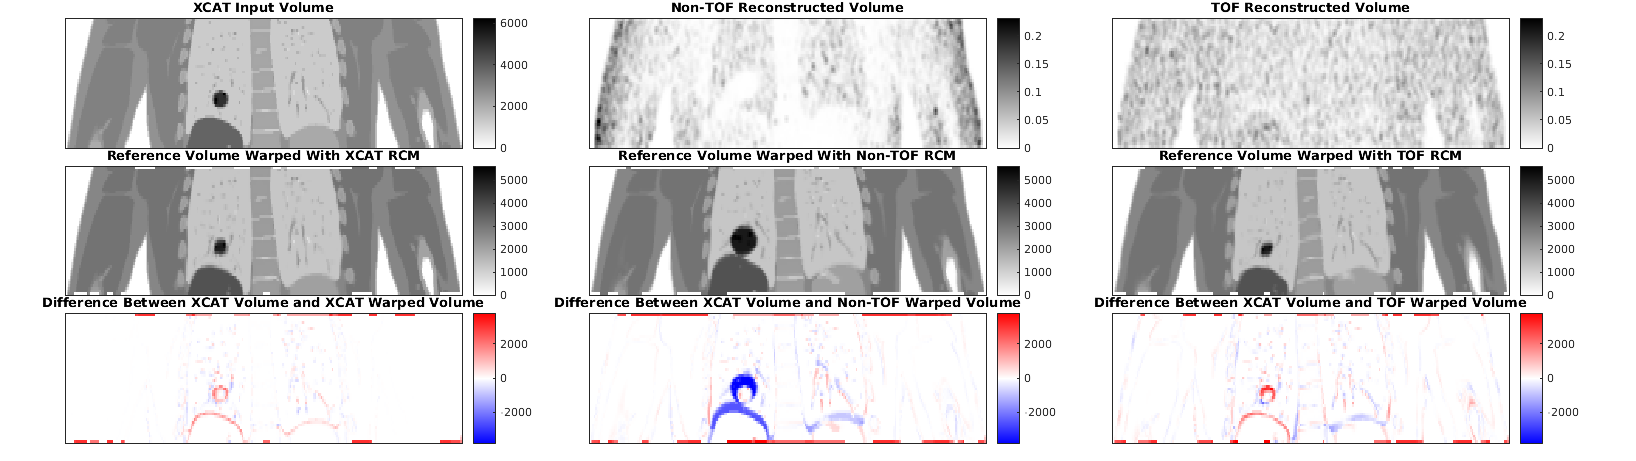
\includegraphics[width=1.0\linewidth]{figures/output.png}
        \captionsetup{singlelinecheck=false, justification=centering}
        \caption{All volumes correspond to end-inhalation. First row from left to right: \gls{XCAT} \gls{PET} data, \gls{NAC} \gls{NTOF} reconstructed data and \gls{NAC} \gls{TOF} reconstructed data. Second row: \gls{RCM} applied to mean position \gls{XCAT} data with \gls{RCM} derived from \gls{XCAT} \gls{PET} data (left), \gls{NAC} \gls{NTOF} (middle) and \gls{NAC} \gls{TOF} (right) volumes. Colour map ranges are consistent for all images on this row. The third row from left to right: The difference between the estimated volumes from the second row with the \gls{XCAT} end-inhalation volume. Colour map ranges are consistent for all images on this row.}
        \label{fig:output}
    \end{figure*}
    
    \begin{figure}[H]
        \centering
        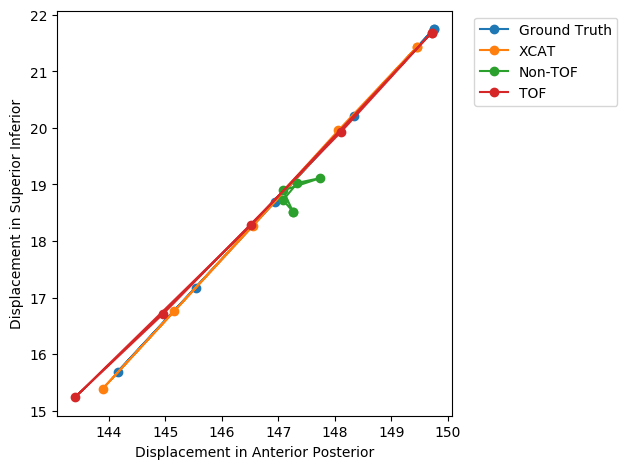
\includegraphics[width=1.0\linewidth]{figures/TOF.png}
        \captionsetup{singlelinecheck=false, justification=centering}
        \caption{The path of the \gls{COM} of the lesion. Horizontal (respectively vertical) axis corresponds to motion in the \gls{AP} (respectively \gls{SI}) direction over the $6$ gates. Different curves denote \gls{COM} displacement for  ground truth data, the estimated data from the \gls{XCAT} based \gls{RCM}, the estimated data from the \gls{NAC} \gls{NTOF} based \gls{RCM} and the estimated data from the \gls{NAC} \gls{TOF} based \gls{RCM}.}
        \label{fig:com_graph}
    \end{figure}
    
     The reconstructed data, estimated volumes and difference can be seen in Fig~\ref{fig:output}. The mean \gls{MAPE} was found to be lower for the \gls{NAC} \gls{TOF} data than for the \gls{NAC} \gls{NTOF}.
    
     \gls{COM} results can be seen in Fig~\ref{fig:com_graph}. The path of the \gls{NAC} \gls{TOF} data follows the ground truth path much closer than the \gls{NAC} \gls{NTOF} data, and is quite close to the gold standard \gls{XCAT}-derived motion.

\section{Discussion and Conclusions} \label{sec:discussion_and_conclusions}
    Motion models derived from \gls{NAC} \gls{TOF} volumes were found to be more robust than when using \gls{NAC} \gls{NTOF}, both visually and when comparing \gls{MAPE} and \gls{COM}. This was noticeable for the lung lesion in the thoracic cavity but also for other parts of the anatomy such as the liver. This is likely due to the improved image contrast of \gls{NAC} \gls{TOF} images.
    
    In the future, research will focus on investigating the robustness of the motion model estimation to different noise levels, acquisition duration and size of lesion.

\AtNextBibliography{\scriptsize}
\printbibliography

\end{document}
